% !TeX encoding = UTF-8
% !TeX spellcheck = lt
\documentclass[a4paper,12pt]{article}
\usepackage[utf8x]{inputenc}
\usepackage[T1]{fontenc}
\usepackage{tabto}
\usepackage{gensymb}
\usepackage{amssymb}

\usepackage[linesnumbered]{algorithm2e}
\renewcommand{\KwData}{\textbf{Duomenys:}}
\renewcommand{\KwResult}{\textbf{Rezultatas:}}
\renewcommand{\algorithmcfname}{Algoritmas}

\usepackage{enumerate}
\usepackage[hmargin={30mm,15mm},vmargin={20mm,20mm},bindingoffset=0mm]{geometry}
\usepackage[onehalfspacing]{setspace}
\usepackage[pdftex,dvipsnames]{xcolor}  % Coloured text etc.
%\definecolor{LinkGray}{gray}{0.30}
\usepackage[colorlinks=true, linkcolor=blue, citecolor=blue, urlcolor=blue, unicode]{hyperref}
\usepackage{amsmath}
\usepackage{graphicx}
\usepackage{float}
\usepackage[section]{placeins}
\usepackage{glossaries}
\renewcommand*{\glsgroupskip}{}
\usepackage{indentfirst}
\usepackage{nameref}
\setlength{\parindent}{4em}
\setlength{\parskip}{0.3em}

%\usepackage{xargs}                      % Use more than one optional parameter in a new commands

\usepackage[colorinlistoftodos,prependcaption,textsize=tiny]{todonotes}
\usepackage{tocloft}
\renewcommand{\cftsecleader}{\cftdotfill{\cftdotsep}} % apply dots in table of contents for sections

\renewcommand{\refname}{Literatūros sąrašas}
\renewcommand{\figurename}{Iliustracija} 
\renewcommand{\contentsname}{Turinys}
\title{Bepiločių orlaivių vietos nustatymas remiantis vaizdine informacija}
\author{Lukas Klusis}

\makeglossaries
\begin{document}
	\sloppy

	\pagenumbering{Roman}
	\thispagestyle{empty}
	\begin{center}
		VILNIAUS UNIVERSITETAS  \\
		MATEMATIKOS IR INFORMATIKOS FAKULTETAS\\
		MATEMATINĖS INFORMATIKOS KATEDRA\\
										
		\vspace{4cm}
		\textbf{Lukas Klusis} \\
		Informatikos studijų programa \\
		Matematinės informatikos šaka\\
		\vspace{3cm}
				    
		\textbf{\Large Bepiločių orlaivių vietos nustatymas remiantis vaizdine informacija}\\
		\vspace{0.5cm}
		\textbf{\normalsize Vision-Based Localization for Unmanned Aerial Vehicles}\\
		\vspace{0.5cm}
		Bakalauro baigiamasis darbas \\
										
		\vspace{6cm}
		Vadovas: \hfill lekt. \textbf{Mindaugas Eglinskas} \hfill \textit{parašas}
		\vfill
		Vilnius \ \ 2015
	\end{center}
	\clearpage
	
	\tableofcontents
	\clearpage
	
		\newglossaryentry{BPO}{name={BPO},description={bepilotis orlaivis}}
		\newacronym{GPS}{GPS}{globali pozicionavimo sistema}
		\newglossaryentry{passivesensor}{name={Pasyvus jutiklis},description={toks jutiklis, kuris nespinduliuoja (nepateikia) jokių duomenų į išorę, o naudoja tik esamą, nepriklausomą nuo jutiklio informaciją }}
		
		\newglossaryentry{opencv}{name={OpenCV},description={\textit{abreviatūra Open Source Computer Vision}, programavimo biblioteka pagrinde skirta darbui su vaizdo apdorojimu}}	
		
		\newglossaryentry{emgu}{name={Emgu},description={biblioteka, kuri įgalina naudoti \gls{opencv} kartu su .NET karkasu}}
		
		\newglossaryentry{csharp}{name={C\#},description={ Objektiškai orientuota programavimo kalba sukurta Microsoft }}
		\newglossaryentry{cpp}{name={C++},description={Objektiškai orientuota programavimo kalba}}
	
		\newglossaryentry{akcelerometras}{name={Akcelerometras},description={prietaisas, kuris išmatuoja pagreitį}}
		\newglossaryentry{gyroscope}{name={Giroskopas},description={prietaisas, skirtas sukimuisi surasti, jį išmatuoti}}
		
		\newglossaryentry{homography}{name={Homografinė matrica},description={Matrica, kuri naudojama susieti du paviršius}}
		
		\newglossaryentry{FLANN}{name={FLANN},description={\textit{abreviatūra, angl. Fast Library for Approximate Nearest Neighbors} - tai yra biblioteka, kuri turi kolekciją algoritmų optimizuotų greitai gretimų ypatybių paieškai dideliuose duomenų kiekiuose, pasiūlytas M. Muja, D. Lowe}}
		
		\newglossaryentry{SIFT}{name={SIFT},description={\textit{abreviatūra, angl. Scale Invariant Feature Transform algorithm}- algoritmas, kuris suranda ir apibūdina paveikslėlio ypatybes, yra nepriklausomas nuo ypatybių mastelio transformavimo, pasiūlytas D. Lowe}}
		
		\newglossaryentry{SURF}{name={SURF},description={\textit{abreviatūra, angl. Speeded Up Robust Features} - algoritmas kuris suranda ir apibūdina paveikslėlio ypatybes}}
				
		\newglossaryentry{FREAK}{name={FREAK},description={\textit{abreviatūra, angl. Fast Retina Keypoint} algoritmas apibūdinantis paveikslėlio ypatybes}}
		
		\newglossaryentry{RANSAC}{name={RANSAC},description={\textit{abreviatūra, angl. Random sample consensus} - algoritmas, kuris iš aibės išmeta išskirtis}}
		
		\newglossaryentry{scene}{name={Scena},description={Žemės paviršiaus žemėlapis, kurio geografinė padėtis yra žinoma}}
		
		\newglossaryentry{model}{name={Modelis},description={Žemės paviršiaus nuotrauka nufotografuota orlaivio kamera}}
		
		\newglossaryentry{imageRegistration}{name={Paveikslėlių registracija},description={Tai procesas, kurio metu dvi skirtingos aibės duomenų yra susiejamos į vieną koordinačių sistemą}}
		
		\newglossaryentry{mercator}{name={Mercator projekcija},description={Flamandų geografo ir kartografo Gerardus Mercator sukurta cilindrinė žemėlapio projekcija}}
		
		\newglossaryentry{WGS84}{name={WGS-84},description={\textit{abreviatūra, angl. World Geodetic System} – Pasaulio geodezinė sistema, tai standartas apibrėžiantis koordinačių sistemą žemės planetai, naudojamas kartografijoje, geodezijoje, navigacijoje, kurios paskutinė versija yra 1984 metų}}	
		
		\newglossaryentry{unimodal}{name={Vienmodalinis skirstinys},description={Skirstinys, kuris turi vieną lokalų maksimumą}}
		\newglossaryentry{multimodal}{name={Multimodalinis skirstinys},description={Skirstinys, kuris turi daugiau negu vieną lokalų maksimumą}}
				
	\clearpage
	\pagenumbering{arabic}
	
	\section*{Įvadas}
		\addcontentsline{toc}{section}{Įvadas}
		Bepiločiai orlaiviai (\gls{BPO}) yra aktyviai naudojami įvairiose srityse ir tikimasi, kad jų panaudojimas stipriai plėsis. Ši technologija yra naudojama tokiose srityse kaip: kelių ar kartografinių žemėlapių sudarymas \cite{RoadDetection12}, žmonių paieškos ir gelbėjimo operacijos \cite{WildernessSearchAndRescue}, karinė žvalgyba ar kovinės operacijos, ūkinės paskirties laukų apžiūra bei priežiūra ir daugelyje kitų sričių.
			
		\subsubsection*{Motyvacija}
			
		Praktiškai visu laikotarpiu, kada naudojama aviacija, egzistavo poreikis bepiločiam skrydžiui. Bepilotis orlaivis yra suprantamas kaip orlaivis, kuris neturi skraidinti piloto ir gali būti valdomas nuotoliniu būdu arba veikti autonomiškai. Dažniausiai bepiločius orlaivius yra siekiama panaudoti kai yra paliečiamas bent vienas iš šių kriterijų: 		
		\begin{itemize}
			\item Rizikingumas - tai užduotys, kuomet yra didelė orlaivio sudužimo ar numušimo tikimybė, kaip pavyzdžiui, karinės užduotys ar skrydžiai virš aktyvių ugnikalnių. Tais atvejais, kai yra pavojus žmogaus sveikatai, pavyzdžiui virš užterštų, kaip pavyzdžiui, skrydžiai virš radioaktyvių ar chemiškai pavojingų zonų. 
			\item Pasikartojančių žmogaus veiksmų eliminavimas - tai skrydžiai, kurių užduotys gali būti automatizuotos, pavyzdžiui, skrydis paskui objektą, paskirtos vietos fotografavimas.
			\item Ekonomiškumas - orlaivis gebantis gabenti žmogų iš principo negali būti mažas, dėl to ir pigus.
			\item Ilgos kelionės - ryškiausi pavyzdžiai būtų kosminiai orlaiviai ar orlaiviai, kurie kaip įmanoma ilgiau sklendžia žemės atmosferoje ir siunčia interneto signalą. 
		\end{itemize}
		
		Anksčiausiai piloto nereikalaujantys skrydžiai buvo panaudoti kariniais tikslais. Išskirtiniu įvykiu galima išskirti Austrijos puolimą 1849 m., kuomet buvo puolamas Italijos miestas Venecija, balionais gabenančiais bombas. Visgi toks skrydis buvo menkai kontroliuojamas, todėl būtina buvo atrasti metodus, kaip valdyti ir aiškiau numatyti bepiločio orlaivio skrydžio rezultatus. Didžiulis proveržis buvo padarytas su radio bangų atradimu ir bepiločių orlaivių kūrimu prasidėjusiu nuo Pirmojo Pasaulinio karo. Kitas svarbus etapas buvo pradėtas su kompiuterių technologine pažanga bei dirbtinio intelekto mokslų srities populiarėjimu. Vienas iš iškeltų tikslų yra įgalinti autonominius robotus, įskaitant ir bepiločius orlaivius, veikti kiek įmanoma labiau autonomiškai. Kartu su BPO autonomiškumo siekimu svarbus elementas tapo gebėjimas patiems orlaiviams nustatyti savo padėtį.
		
		Egzistuoja dvi padėties nustatymo klasifikacijos. Pirmoji, kai orlaivis nustato savo vietą lokaliai, t. y. orlaivio pozicija yra skaičiuojama nuo lokalaus, dažniausiai tik šiam orlaiviui žinomo atskaitos taško, pavyzdžiui nuo skrydžio pradžios taško. Antrasis variantas yra, kuomet orlaivis savo vietą susieja su globaliu, standartiniu atskaitos tašku, pavyzdžiui, žemės centru.
		
		\subsubsection*{Problemos aprašymas}
					
		Daugelyje globalaus pozicionavimo reikalaujančiuose sprendimuose yra naudojama \acrfull{GPS}. Tai yra Jungtinių Amerikos Valstijų (JAV) Saugumo Departamento sukurta sistema. Sistema pradėta kurti 1973 m., o pilnai veikia nuo 1995 m. ir susideda iš dviejų pagrindinių dalių: 24 aplink žemę skriejančių dirbtinių palydovų ir žemės paviršiuje esančių GPS imtuvų, kurie iš gaunamų palydovų signalų geba apskaičiuoti savo poziciją. Nors egzistuoja GPS alternatyvų, kaip Rusijos Globali Navigacinių Palydovų Sistema (GLONASS) ar planuojama Europos Sąjungos Galileo pozicionavimo sistema, tačiau šių sistemų veikimo principas yra analogiškas GPS todėl šio darbo metu, paprastumo dėlei yra vertinama tik GPS įtaka.   
				
		Būtinybę bepiločiams orlaiviams turėti pastovų kontaktą su GPS palydovais yra didelis trūkumas urbanistinėse vietovėse, kur, dėl pastatų blokuojamo GPS signalo, teikiama paklaida gali būti didesnė negu keliasdešimt metrų \cite{GPSAccuracyInCity}. Ne retu atveju, tokio dydžio paklaida, gali būti lemiamas veiksnys apribojantis bepiločio orlaivio panaudojimą.
		Iš kitos pusės GPS sistemą negalima laikyti patikima \cite{GpsVulnerability}, naudojant sąlyginai nebrangius prietaisus įmanoma „užteršti“ GPS signalo kanalą, taip niekados neleidžiant prietaisui nustatyti savo pozicijos ar net apgauti GPS imtuvus, taip kad teikiami rezultatai būtų parinkti kito asmens. Toks navigacinės sistemos pažeidžiamumas yra aktuali problema konfliktinėse zonose, stipriai apribojanti bepiločių orlaivių galimybes.
		Egzistuoja ir kitos priežastys, dėl kurių verta kurti nepriklausomą navigacinę sistemą. Po 2001 m. rugsėjo 11-tosios įvykių, kuomet teroristai įvykdė išpuolį prieš JAV, buvo paskatintos diskusijos, dėl visos GPS sistemos nenutrūkstamo prieinamumo katastrofinių situacijų metu. Galima daryti tik vieną išvadą - negalima garantuoti, kad GPS palydovai, o kartu ir jų siunčiamas signalas visada bus pasiekimas.
				
		Nagrinėjant toliau, GPS sistema šiuo metu yra galima tik žemės planetoje, dėl to reikia toliau ieškoti naujų navigacijos būdų, kuriais remiantis būtų galima naviguoti kituose kosminiuose objektuose - planetose, palydovuose, kometose.
				
		\subsubsection*{Vaizdo medžiaga pagrįsti sprendimai}

		Suvokiant visus šiuos GPS sistemos trūkumus yra ieškoma būdų, kaip nustatyti orlaivio vietą nesinaudojant jokiais papildomais išoriniais davikliais. Vienas iš tokių variantų yra vietos nustatymas, naudojant vaizdo kamerą. Tai yra tapusi viena iš aktualiausių tyrimų sferų bepiločių orlaivių ir visos robotikos srityje. Vaizdo kamera yra labai patraukus pasirinkimas dėl pigios kainos bei vis didėjančių tyrimų vaizdo paremtuose pozicionavimo sprendimuose, kurie įgijo didelį  dėmesį, kuomet tapo įmanoma skaičiavimo galimybes perkelti į patį orlaivį. 
		Galima išskirti daugiausiai dėmesio sulaukusius sprendimus. Pirmiausia, tai yra vizuali odometrija, kuomet roboto pozicija ir orientacija yra nustatoma analizuojant gretimus kameros paveikslėlius. Šis metodas yra pritaikytas tokiose sudėtingose operacijose, kaip Marsaeigių vietos nustatymui. Kita didelio dėmesio sulaukusi sritis yra dviejų vaizdo paveikslėlių susiejimas arba kitaip tariant \glslink{imageRegistration}{paveikslėlių registracija}. Tai ypač aktualu vietos nustatymui, turint mintyje, kad yra daug viešų servisų, kaip \textit{Microsoft Bing Maps} ar \textit{Google Maps}, kurie teikia pasaulio žemėlapius su žinomomis koordinatėmis.
		
		\subsubsection*{Tikslas ir uždaviniai}
		Šio darbo tikslas yra sukurti sistemą - grupę susijusių ir kartu dirbančių dalių - kuri, remiantis vaizdo kameros ir paveikslėlių, kurių žinoma geografinė padėtis, registracija, gebėtų nustatyti orlaivio poziciją.  		
		Šiam tikslui įgyvendinti yra apžvelgiama literatūra, parenkami gali sprendimo būdai bei šie būdai yra eksperimentiškai patikrinami. 
						
		\subsubsection*{Panašūs darbai}
		
		Yra atliktų kitų, panašių darbų. Vienas tokių yra \cite{VisualTrackingAndNavigation}. Darbe yra siūloma navigacinė sistema skirta BPO, kuri gali sekti judantį objektą be GPS sistemos. Tai yra atliekama analizuojant vaizdo kadrų seką ir nustatant sekamo objekto pikselių koordinates, kuriomis vadovaujantis yra toliau naviguojamas orlaivį paskui šį objektą. Kitų bandymų metu \cite{Con:2009:214103} yra siūloma navigacinė sistema, kuri apjungia vizualią odometriją ir žemėlapių, kurių žinoma geografinė padėtis, registraciją su gaunamu vaizdu. Atlikus registracijai gauti duomenys yra filtruojami naudojant taškų masės filtrą bei galiausiai duomenys sujungiami naudojant Kalman filtrą, tokiu būdu, kaip galutinis rezultatas, yra apskaičiuojamos koordinatės \gls{WGS84} koordinačių sistemoje. 
			 
 		\pagebreak	
\section{Apžvalga}		
	\subsection{Inercinė navigacija}
		\label{sec:InertionNavigation}
				
		Vienas iš pagrindinių navigacinės sistemos komponentų yra inercinė navigacinė sistema (INS). INS yra rinkinys pasyvių jutiklių, kuriuos dažniausiai sudaro \glslink{akcelerometras}{akcelerometras} ir \glslink{gyroscope}{giroskopas}, kurie teikia tokius duomenis kaip greitis, posūkio kampas. INS duomenis skaičiuoja remdamasi savo paties pateiktais ankstesniais duomenimis, todėl, kad ir nedidelės paklaidos, laikui bėgant ji vis didėja, Tai yra pagrindinė priežastis, kodėl INS dažniausiai nėra naudojama kaip viena sistema, kartu naudojami papildomi jutikliai kaip barometras orlaivio aukščio patikslinimui, kompasas posūkio kampo patikslinimui, bei kiti jutikliai ar naudojama vizuali odometrija tiek greičio, tiek posūkio kampo nustatymui.	
			
	\subsubsection{Vizuali odometrija}
		\label{sec:VisualOdometry}
			
		Vizuali odometrija yra tapusi populiaria tema, atlikti bandymai rodo, kaip ją praktiškai galima pritaikyti \gls{BPO} vietos nustatymui	\cite{SVO:FastVisualodOmetry}.  Šio darbo metu pilnas vizualios odometrijos funkcionalumas nebus realizuotas, nors tai didelė ir perspektyvi sritis tobulinimui ateityje. Šio darbo vienas iš svarbiausių veiksnių, nuo kurio labai stipriai priklauso vaizdu paremtos vietos nustatymas yra žinojimas, kokiu kampu pasisuko orlaivis dvimatėje erdvėje per laiką \textit{t}.
			
		Šiam poreikiui įgyvendinti galima remtis tiek inercinės navigacijos teikiamais duomenimis, tiek išsiskaičiuoti kampą remiantis vizualios odometrijos principais. Būtent pastarasis variantas čia aprašomas. Turint paveikslėlį, kuris gautas esamu skrydžio metu ir paveikslėlį, kuris buvo užfiksuotas prieš laiką \textit{t} galima nustatyti \glslink{homography}{Homografinę matricą}, kuri sieja šiuos paveikslėlius, svarbu užtikrinti, kad laikas \textit{t} nebūtų per didelis ir paveikslėliai turėtų pakankamai didelį kiekį bendrų taškų. Pavyzdys tokio sulyginimo yra pavaizduotas iliustracijoje \ref{fig:Homography}. Tai galima padaryti atlikus šiuos žingsnius:
		\begin{enumerate}[1.]
			\setlength\itemsep{0em}
			\item Aptinkamos paveikslėlių ypatybės abiejuose vaizduose. Tai gali būti įvairūs taškai, linijos, kampai ar kiti objektai. Dažniausiai naudojami \gls{SURF}, \gls{SIFT} ar kiti algoritmai.
			\item Ištraukti ir aprašyti paveikslėlių ypatybes, tai galima padaryti naudojant \gls{SURF}, \gls{SIFT}, \gls{FREAK} ar kitus algoritmus.
			\item Sugrupuoti ištrauktas paveikslėlių ypatybes, tai dažniausiai daroma brutalios jėgos arba \gls{FLANN} algoritmu.
			\item Sugrupuotų paveikslėlių ypatybės gali turėtų pakankamai daug neteisingai sugrupuotų taškų, todėl galiausiai yra pritaikomas \gls{RANSAC} algoritmas, kuris išfiltruoja taškus – išskirtis ir apskaičiuojama \glslink{homography}{homografinė matrica}.
		\end{enumerate}
		Turint homografinę matricą galima ją išskaidyti į posūkių, postūmių matricas ir normalės vektorių \cite{malis:inria-00174036}.
				
		\begin{figure}[h]
			\includegraphics[width=\textwidth]{images/HomographyMatrix.png}
			\caption{Homografinės matricos suradimas tarp kadrų, kuriuos skiria nedidelis laiko tarptas \textit{t}.}
			\label{fig:Homography}
		\end{figure}				
		
			\subsection{Žemėlapio sudarymas}
			\label{sec:CreationOfMap}
			
			Konstruojant žemėlapį, yra naudojama \gls{mercator} projekcija, bei daroma, prielaida, kad žemė yra tobulo rutulio formos. Taip yra supaprastinamas žemėlapių konstravimas bei jo manipuliavimas, tačiau naudojant ilgumos ir platumos koordinates yra daroma prielaida, kad jos yra \gls{WGS84} standarto.
			
			Visas pasaulio žemėlapis yra suskaidomas į 256 x 256 pikselių kvadratėlius, o jų kiekis priklauso nuo žemėlapio detalumo lygio.
			Detalumo lygis vienareikšmiškai apibrėžia kokio pločio ir aukščio (pikseliais) yra žemėlapis:	
			\begin{equation}
			\textit{žemėlapio dydis} = \textit{žemėlapio aukštis} = \textit{žemėlapio plotis} = 256 \times 2^\textit{detalumo lygis } \left(\textit{pikselių}\right)
			\end{equation}
			\begin{equation}
			\textit{žemėlapio rezoliucija} = \cos({\frac{platuma \times \Pi}{180}}) \times \frac{{den} \textit{žemės spindulys}}{\textit{žemėlapio dydis}} \left(\frac{metrai}{pikselyje}\right) 
			\label{eq:MapResolution}
			\end{equation}		
			
			Žemėlapio pikseliai yra skaičiuojami nuo viršutinio, kairio kampo (0,0) iki apatinio dešinio kampo (\textit{aukštis, plotis})		
			
			Kiekvienam žemėlapio kvadratėliui yra suteikiamas kodas sudarytas iš 4 simbolių abėcėlės: \textit{0, 1, 2, ir 3}. Kodas sudaromas tokia tvarka: pirmo detalumo lygio žemėlapis padalijamas į 4 dalis, joms paeiliui priskiriami simboliai iš abėcėlės, gaunami pirmo lygio kvadratėlių raktų kodai. Kiekvieną iš gautų 4 kvadratėlių vėl dalijame į 4 lygias dalis ir kiekvienai iš šių dalių paeiliui prie esamo kodo pridedame simbolį iš abėcėlės, taip gausime aukštesnio detalumo lygio kvadratėlių kodus. Kartojant šiuos veiksmus galime sudaryti kaip norimai detalaus žemėlapio kvadratėlių raktų kodus. Kodų sudarymas yra pavaizduotas iliustracijoje \ref{fig:quadkey}. Šis kodas pasižymi gera savybė - kodo ilgis yra lygus žemėlapio detalumo lygiui.
			
			\begin{figure}[h]
				\includegraphics[width=\textwidth]{images/MapZooming.png}
				\caption{Žemėlapio kvadratėlių kodų sudarymas}
				\label{fig:quadkey}
			\end{figure}
			
			Turimą ilgumą ir platumą galima konvertuoti žemėlapio pikselių koordinates:	
			\begin{equation}
			\text{pikselio x koordinatė} = \frac{ilguma + 180}{360} \times \text{žemėlapio dydis}
			\end{equation}	
			\begin{equation}	
			\text{pikselio y koordinatė} = 0,5 - \log \left(\frac{1+\sin \left(platuma \times \frac{\Pi}{180}\right)}{1-\sin \left(platuma \times \frac{\Pi}{180}\right)}\right) \times \frac{1}{4\Pi} \times \text{žemėlapio dydis}
			\end{equation}	
						
			Taigi žinant vieną iš šių variantų	galima lengvai ir vienareikšmiškai apibrėžti žemėlapio poziciją bei apskaičiuoti likusius variantus:
			\begin{enumerate}[(a)]
				\item kvadratėlio rakto kodą ir lokalias pikselio koordinates tame kvadratėlyje,
				\item globalaus (viso pasaulio žemėlapio) pikselio koordinates ir detalumo lygį,
				\item ilgumos ir platumos koordinates bei detalumo lygį.
			\end{enumerate}	
		
	\subsection{Paveikslėlių registracija}
		\label{sec:ImageRegistration}
		Paveikslėlių registracija, tai procesas, kurios metu yra surandamas geometrinių transformacijų sąryšis tarp dviejų paveikslėlių duomenų poaibių.
	
		Tariama, kad \gls{scene} ir \gls{model} yra du skirtingi paveikslėliai, užfiksuoti skirtingu laiku, kameros pozicija, posūkio kampu bei pačia kamera, tačiau fiksuojama vieta fiziškai arti, iš tiesų, scenos geografinė aprėptis yra didesnė negu modelio.
	
		Egzistuoja daug sprendimo variantų, kaip scenoje atrasti modelį. Visi jie skirtingai reaguoja į scenos ir modelio mastelio, posūkio kampų, spalvų, jutiklių (kameros) skirtumus, taip pat jų skaičiavimo trukmė yra labai skirtinga.
				
	\subsubsection{Ypatybių atitikmens būdas}
		
		Vienas iš paprasčiausių variantų yra pritaikyti SIFT ar kitus paveikslėlio ypatybių išskyrimo ir sugrupavimo algoritmus, kurie jau buvo aprašyti skyriuje \nameref{sec:VisualOdometry}. Šis algoritmas nėra priklausomas nuo paveikslėlių mastelių, pasukimo kampų, yra sąlyginai greitas, tačiau šis algoritmas yra ganėtinai jautrus apšvietimo pasikeitimui, skirtingų jutiklių naudojimui.
		
	\subsubsection{Kontūrų atitikmenų būdas}
		
		\begin{figure}[h]
			\centering
			\includegraphics[width=0.8\textwidth]{images/ContourMatches.png}
			\caption{Scenos (kairėje) ir modelio (dešinėje) kontūrų grupavimas}
			\label{fig:ContourMatching}
		\end{figure}
		
		Kitas būdas yra ryškiausių kontūrų išskyrimas ir jų lyginimas. Kontūru vadiname aibę taškų, kurie paeiliui apibrėžia kreivę. Ši kreivė dažniausia yra padaroma iš objekto kampų ir linijų, tai dažniausiai yra objekto paveikslėlyje ribos. Paieškos globaliame žemėlapyje atveju yra tariama, kad tiek scenoje, tiek modelyje egzistuoja diskrečių, pakankamai didelių objektų, pavyzdžiui: namas, ežeras, sala, aikštelė ar panašus objektai, kurie gali būti apibrėžti kontūru. Ištraukus apibrėžtus kontūrus tiek apie scenos, tiek apie modelio ryškiausius objektus, reikia juos sugrupuoti, grupavimo pavyzdys pavaizduotas iliustracijoje \ref{fig:ContourMatching}. Grupavimo būdai yra aprašyti darbuose \cite{ Abbasi99, cui2009curve, wang20072d}. Atlikus kontūrų grupavimą, reikia nustatyti modelio padėti scenoje, tam naudojamas \gls{RANSAC} algoritmas.
		Sulyginti scenos ir modelio mastelius, galima papildomai vertinti kontūrus pagal plotą ar perimetrą.
				
	\subsubsection{Šablono atitikmenų būdas}
		\label{sec:TemplateMathing}
		Šablono atitikmenų paieška (arba šablono poravimas) yra technika, kuria ieškoma dalies paveikslėlio (modelio) didesniame paveikslėlyje (scenoje). Šablonų poravimas yra atliekamas modelio paveikslėlį paeiliui lyginant su scenos paveikslėlio dalimi. Pradedant nuo viršutinio kairio kampo yra paskaičiuojama įvertis, kiek scenos dalis, prasidedanti nuo šio taško sutampa su modeliu. Toks įvertis yra paskaičiuojamas kiekviename scenos taške „slenkant“ po vieną pikselį į šoną ar apačią, kol tik įmanoma sudaryti modelio dydžio paveikslėlio poaibį. Atitikimo įvertinimą galima skaičiuoti keletą metodų, šio darbo metu yra naudojamas normalizuotos kryžminės koreliacijos metodas, kurį galima aprašyti lygtimi:
		\begin{equation}
		C(x,y) = \frac{\sum_{(x_1,y_1) \in M} \left( M(x_1,y_1) \cdot S(x+x_1, y + y_1) \right)}
		{\sqrt{\sum_{(x_1,y_1) \in M} M(x_1,y_1)^2 \cdot \sum_{(x_1,y_1) \in M} S(x+x_1, y + y_1)^2  }}
		\label{eq:TemplateMatching}
		\end{equation}	
		
		čia $M$ yra modelio, o $S$ scenos paveikslėliai. Suskaičiavus, kiekvienam galimam taškui jo atitikimo įvertį, gausime $(w_s-w_m+1) \times (h_s-h_m+1)$ (čia $w_s$ ir $h_s$ bei $w_m$ ir $h_m$ yra atitinkamai scenos ir modelio pločiai bei aukščiai) taškų, kurių vertės yra nuo 0 iki 1, šių taškų aibę žymime 
		\begin{equation}
		C =  \{\; \langle x, y, C(x,y) \rangle \; \textbar \; 0 \leq x \leq w_s-w_m+1, 0 \leq y \leq h_s-h_m+1\}
		\end{equation}
		Svarbiausias yra taškas, kurio vertė didžiausia, pažymėkime jį $C_{max}$ tačiau dėl per laiką pakitusio žemės reljefo, apšvietimo sąlygų ar kitų veiksnių, dažnai negalima remtis tik didžiausio taško suradimu, todėl yra įvedamas parametras $c^- \in (0;1]$, kuris atlieka slenksčio funkciją, t.y. iš aibės $C$ išrenkame taškus
		\begin{equation}
		\label{eq:TemplateMathingFilteredResult}
		 F = \left\{\; \langle x, y, c \rangle \; \textbar \; \langle x, y, c \rangle \in C  \; \land \; c \geq c^- \cdot C_{max} \; \land \; (x,y)\text{ yra lokaus maksimumo taškas} \right\}
		\end{equation}
		Kitaip tariant, aibės $F$ elementus vadinsime šablonų poravimo kandidatais, t. y. taškai scenoje ir jų įvertis $c \in [0;1]$ kiek tiksliai šablonas atitinka scenos vietą. Kadangi tikrasis atitikmuo gali būti ne daugiau negu 1 kartą, vadinasi aibėje F yra mažiausiai $|F| - 1$ klaidingų sutapatinimų. 
		
		Aibės $C$ taškus galima interpretuoti kaip atskirą paveikslėlį, iliustracijoje \ref{fig:TemplateMatchesRaw} pateiktas pavyzdys, šviesesni taškai reiškia stipresnį sutapimo įvertį, šį paveikslėlį vadinsime Atitikmenų paveikslėliu. Toks duomenų interpretavimas suteikia papildomų galimybių, pavyzdžiui klaidų mažinimui. Galima pritaikyti plačiai žinomus vaizdo apdorojimo algoritmus.		
				
	\subsection{Lokalizacija}	
		\label{sec:Localization}
				
		Šiame skyriuje yra apjungiamos visos sistemos dalys į vieną bendrą algoritmą. 
		Apie vietos nustatymo principus ir algoritmus kalbama knygose \cite{siegwart2011introduction, thrun2005probabilistic}. Šio darbo metu yra naudojami dviejų tipų \hyperref[sec:BayesFilter]{Bayes filtrai}: \nameref{sec:KalmanFilter} (detaliau aprašomas darbe \cite{DesignEKF}) ir \nameref{sec:ParticleFilter} (detaliau aprašomas darbe \cite{BaBl09}). 
						
		Lokalizacija stipriai remiasi tikimybinių skirstinių sudarymu bei aplinkos sąveikomis.		
		Aplinkos parametrai yra apibrėžiami kaip \textit{būsena}. Būsena galima suprasti kaip $n-dimensijų$ kintamąjį, kuris kinta laiko $t$ atžvilgi ir kuriuo apibrėžiami orlaivio fizikiniai parametrai, pavyzdžiui vieta, pagreitis, kitaip tariant, būsena yra elementas iš aibės 
		\begin{equation}
			\label{eq:statesSet}
			\mathbb{S} = \left\{ \langle s_1, s_2,\dots, s_n \rangle \;\textbar\; i= \overline{1..n}, s_i \in S_i \right\}
		\end{equation}
		kur kiekviena aibė $S_i$ simbolizuoja būsenos dedamąją dalį, kurios dažnai būna:
		\begin{itemize}
			\item pozicija - tai dažniausiai viena, dvejom arba trimis dimensijomis apibrėžia orlaivio vietą sutartoje koordinačių sistemoje.
			\item greitis - tai viena, dvejom arba trimis dimensijomis apibrėžia kokiu greičiu kinta orlaivio pozicija sutartoje koordinačių sistemoje.
			\item orlaivio kampas - taip pat vienam dejom arba trimis dimensijomis apibrėžia kokiu kampu pasisukęs orlaivis.
		\end{itemize}
		Galima būsena apibrėžti ir daugeliu kitų būsenos parametrų.
		
		Pagrindine idėja yra nustatyti orlaivio būseną remiantis jutiklių duomenimis. Jutiklių duomenys gali būti tik daliniai bei taip pat jų matavimai gali būti atlikti su tam tikra paklaida - triukšmu. Užuot stengiantis išmatuoti tikslią vienintelę būseną, ji yra skaičiuojama kaip tikimybinis būsenų skirstinys, kuris yra vadinamas įsitikinimu, kuris aprašytas toliau (\ref{eq:belief}).
		
		Svarbūs standartiniai žymėjimai $x_{t_1:t_2},\, z_{t_1:t_2},\, u_{t_1:t_2}$, detalesnius jų aprašymus galima rasti knygoje  \cite{thrun2005probabilistic}(p. 16 - 32). Tai yra daugia-dimensiniai kintamieji, kurie šio darbo metu yra apibrėžti aibėje $\mathbb{S}$.

		\begin{itemize}
			\item būsenų aibė, kurioje yra orlaivis per laiką $(t_1;t_2]$, ($t_1 \leq t_2$):
				\begin{equation}
					x_{t_1:t_2} = x_{t_1}, x_{t_1+1},\dots,x_{t_2} 
				\end{equation}
			\item aibė matavimų duomenys, kurie sako, kokioje būsenoje yra orlaivis per laiką $(t_1;t_2]$, ($t_1 \leq t_2$):
				\begin{equation}
				z_{t_1:t_2} = z_{t_1}, z_{t_1+1},\dots,z_{t_2} 
				\end{equation}
			\item $u_{t_1:t_2}$ - kontroliniai, judesio duomenys. Tai yra informacija kaip pasikeitė būsena per laiką $(t_1;t_2]$, ($t_1 \leq t_2$):
				\begin{equation}
				u_{t_1:t_2} = u_{t_1}, u_{t_1+1},\dots,u_{t_2} 
				\end{equation}
		\end{itemize}	

		Svarbios dvi tikimybinės lygtys:
		\begin{itemize}
			\item $p(z_t|x_t)$ - matavimo tikimybė. Dažnai gali nepriklausyti nuo laiko parametro $t$, t.y $p(z_t|x_t) = p(z|x), \forall t$. Kitaip tariant, tai orlaivio pozicija nustatyta, remiantis jutiklių informacija su triukšmu.
			\item $p(x_t|x_{t-1},u_t)$ - būsenos pakitimo tikimybė. Ši tikimybė rodo, kur tikėtiniausia yra orlaivis laiko momentu $t$, žinant kad orlaivis atliko $u_t$ veiksmus.
		\end{itemize}	
			
		Vietos nustatymas nėra vienareikšmis procesas, kurio metu būtų galima garantuotai nusakyti orlaivio vietą. Orlaivis remiantis jutiklių duomenis gali įvertinti tik savo pozicijos tikimybę, kuri yra vadinama \textit{įsitikinimu}. Įsitikinimas dažniausiai yra reprezentuojamas tikimybinių skirstiniu. Šio darbo metu tokius įsitikinimus galima apibrėžti funkcija iš aibės:
		\begin{equation}
			\mathbb{B} = \left\{bel \;\textbar\; bel: \mathbb{S} \rightarrow [0;1]^n, \sum_{x \in \mathbb{S}}bel(x) = 1 \right\}
		\end{equation}
		čia funkcijos \textit{bel} pavadinimas yra kilęs iš angliško žodžio \textit{belief - įsitikinimas}. 
		
		Įsitikinimą, galima išreikšti tikimybine priklausomybe:	
		\begin{equation}
			bel(x_t) = p(x_t | z_{1:t}, u_{1:t})
			\label{eq:belief}
		\end{equation}
		Kas kitais žodžiais reikštų, kokia tikimybė, kad robotas vietoje $x_t$, kai yra žinomi matavimų $z_{1:t}$ ir atliktų judesių $u_{1:t}$ duomenys
		
		Pagal šią lygtį (\ref{eq:belief}) įsitikinimą galima apskaičiuoti tik žinant  to laiko matavimų įvertinimą $z_t$. Dažnai yra naudinga apskaičiuoti įsitikinimą prieš atliekant matavimus ir ką tik atlikus judesius. 
		\begin{equation}
			\overline{bel}(x_t) = p(x_t | z_{1:t-1}, u_{1:t})
		\end{equation}
		Tikimybinis skirstinys $\overline{bel}$ dažnai yra vadinamas \textit{prognozė}. O apskaičiavimas $bel$ žinant $\overline{bel}$ yra vadinamas \textit{korekcija} arba  \textit{matavimo atnaujinimas}. 
			
		Kadangi dažniausiai įsitikimas būna pasiskirstęs pagal Gauso skirstinį, paprastumo dėlei darome prielaidą, kad įsitikinimas, negali turėti dviejų taškų, kurie yra maksimumo taškai. 
		Tada tašką, kuriame įsitikinimas įgyja maksimalią reikšmę vadiname įsitikinimo pozicija:
		\begin{equation}
			pos(bel) = x \in \mathbb{S}, \; kur \; bel(x) = \max_{x' \in \mathbb{S}}{bel(x)}
		\end{equation}
		
		Yra keli variantai, kaip galima reprezentuoti roboto įsitikinimą - vienos hipotezės arba daugelio hipotezių įsitikinimu. Vienos hipotezės įsitikinimo atveju yra skaičiuojamas vienas unikalus taškas, ar tiksliau - įsitikinimas,  žemėlapyje. Šis principas remiasi sąlyga, kad iš gaunamų duomenų apskaičiuota pozicija duoda vienintelį rezultatą, t. y. nesukelia pozicijos neaiškumų. Toks būdas yra įmanomas turint jutiklius, kurių duomenys su paklaida yra pasiskirsčiusi pagal Gauso skirstinį, tokius jutiklio duomenis galima suvesti į vieną tašką, pavyzdžiui, inercinės navigacinės sistemos, ar vizualios odometrijos atvejais. Visgi vienos hipotezės atveju dėl jutiklių triukšmo ar judesių kontrolės netikslumų toks duomenų sutraukimas į vieną tašką tampa sudėtingu, turintis didelį neapibrėžtumą, kuris laikui bėgant padaro galutinį rezultatą praktiškai nepanaudojamą. Tuo labiau, tais atvejais, kai duomenys yra „šuoliuojantys“, t. y. jutiklis gali pateikti rezultatus, kurie turi daugiau negu vieną lokalaus maksimumo tašką, kitaip tariant yra pasiskirstę ne pagal Gauso skirstinį, vienos hipotezės įsitikinimas tampa išvis neįmanomas. Pastaroji situacija yra kuriama ir paveikslėlių registracijos metu, todėl šio darbo metu, būtina remtis daugelio hipotezių įsitikinimu. Daugelio hipotezių atveju, bepilotis orlaivis seka, ne tik vieną, bet taip pat ir galimai begalinę aibę įsitikinimų:
		\begin{equation}
			Bel = \left\{ bel_i \; \textbar\;  i = \overline{1...n},n \in \ \mathbb{N}\; \land \;  bel_i \in \mathbb{B} \right\}
		\end{equation}
	
		Turint daug galimų hipotezių, labai svarbu nustatyti tam tikrą įsitikinimų rikiavimą. Tam tikslui konstruojama svorinė pozicijų aibė: 
		\begin{equation}
		Bel_w = \left\{ \langle bel_i, w_i \rangle \; \textbar\;  w_i \in [0,1], \; bel_i \in Bel \; \forall i \right\}
		\end{equation}
		T. y. įvertinant tam tikrus faktus galimoms pozicijoms yra suteikiama tikimybė. Kaip šios tikimybės suteikiamos bus aiškinamasi vėliau. Toks įsitikinimų suskirstymas remiasi dvejais teiginiais:
		\begin{enumerate}[1.]
			\item gali egzistuoti ne daugiau kaip vienas tikrasis įsitikinimas.
				Įsitikinimas vadinamas tikruoju (teisingu) jeigu jo pozicija yra nutolusi nuo fizinės vietos, kurioje egzistuoja orlaivis per sąlyginai nereikšmingą atstumą. Bandymų metu tokiu atstumu buvo laikyti 2 metrai. Visi kiti įsitikimai vadinami netikrais (neteisingais).
			\item rekursyviai atjauninant įsitikinimą, tikimasi, kad gauti duomenys patvirtins tikrojo įsitikinimo poziciją (padidins įsitikinimo tikimybe), o netikrų įsitikinimų tikimybė bus mažinama.
		\end{enumerate}
				
		\subsubsection{Bayes filtras}
		\label{sec:BayesFilter}
		
		Bayes filtras, dar vadinamas rekursyviu Bayes filtru yra algoritmas, kuris yra tapęs, kaip karkasas daugeliui navigacijos praktikoje naudojamų algoritmų. 
		Tai yra rekursyviai veikiantis algoritmas, kuris susideda iš dviejų esminių dalių:
		\begin{enumerate}
			\item Prognozė - Šiuo žingsniu yra apskaičiuojamas įsitikinimas $\overline{bel}(x_t)$ laiko momentų $t$, kuomet yra žinomas įsitikinimas $bel(x_{t-1})$ laiko momentu $t-1$ bei atlikti kontroliniai (judesio) veiksmai $u_t$.
			\item Taisymas - tai yra prognozės korekcija atsižvelgiant į matavimų tikimybę.
		\end{enumerate}
		
		Dažniausiai Bayes filtras praktikoje nėra naudojamas, tačiau dvi šio filtro implementacijos - Kalman \cite{siegwart2011introduction, thrun2005probabilistic} ir Dalelių filtrai \cite{Gustafsson2010} yra apžvelgiami toliau.
		
		Šie algoritmai skiriasi, su kokiais tikimybiniais skirtiniais gali dirbti.	
				
		Kalman filtras yra ne kartą patvirtinęs, kad yra patikimas algoritmas jutiklių duomenų filtravimui. Tačiau Kalman filtras gali būti pritaikomas, tik tada, kai matavimų duomenys yra pasiskirstę pagal Gauso skirstinį. Yra pasiūlyta \cite{JulierUhlmann2004} Kalman filtro variacijų duomenims pasiskirsčiusiems ne pagal Gauso skirstinį, tačiau reikalaujama, kad skirstinys būtų \glslink{unimodal}{vienamodalinis}. Priešingai šiai situacijai yra dalelių filtras, kuris gali dirbti su \glslink{multimodal}{multimodaliniais} skirtiniais.
				
		\subsubsection{Dalelių filtras}
		\label{sec:ParticleFilter}
		
		Visa dalelių filtro idėja yra reprezentuoti orlaivio poziciją aibe pavyzdžių, pasiskirsčiusiu po turimą žemėlapį. Tada kiekvieną iš šių dalelių atnaujinti kartu su iš jutiklių gaunamais duomenimis ir įvertinus šių dalelių tikėtinumą, palikti tik tikėtinas daleles, taip apytiksliai nustatoma orlaivio pozicija žemėlapyje. Dalelių filtrą galima suskirstyti į 3 dalis: 1. Dalelių pozicijos „paslinkimą“, pagal jutiklių duomenis; 2. Dalelių pasvėrimą; 3. Dalelių išrinkimą. Algoritmas detaliai pavaizduotas (\ref{alg:pf}).		
		
		Dalelių filtro algoritme yra naudojama aibė mėginių - dalelių, kur kiekviena dalelė yra konkreti hipotezė teigianti, kad orlaivis yra nurodytoje vietoje:
		\begin{equation}
		\chi_{t} := \left\{x_{t}^{[1]},\, x_{t}^{[2]}, \dots ,x_{t}^{[M]} \right\} \subset \mathbb{S}
		\end{equation}
		
		Daleles pirmai iteracijai sugeneruojame pasinaudoję šablonų poravime gautu aibės $F$ (\ref{eq:TemplateMathingFilteredResult}) rezultatu, bei aplink šiuos taškus paskirstomos dalelės pagal Gauso skirstinį.
		
		\begin{algorithm}[h]
			\label{alg:pf}
			\SetNlSty{}{}{:}
			\LinesNumbered
			
			\KwData{ Aibė dalelių laiko momentu $t-1$: $\chi_{t-1}$, judesio duomenys: $u_t$, matavimų duomenys: $z_t$\\}
			\KwResult{ Aibė dalelių laiko momentu $t$: $\chi_{t}$ \\}		
			$\overline{\chi_{t}} = \chi_{t} = \varnothing$\;
			\ForEach{dalelė $x_{t-1} \in \chi_{t-1}$}
			{		
				\tcp{1. Dalelių paslinkimas:}
				$m = \min\left\{\frac{|\chi_{t-1}|}{N_{max}}, Random(1,inc)\right\}$ \label{alg:pf:HowManyProjectionstoMake} \;
				parinkti pavyzdžius $\overline{\chi_{t}}' = \{ x_t^{[1]},\, x_t^{[2]},\, \dots, x_t^{[m]}\} \sim p(x_t \,|\, x_{t-1}, u_t)$  \label{alg:pf:MakeProjection}\;
				
				\tcp{2. Nustatomi dalelių svoriai:}
				\ForEach{dalelė $x_t \in \overline{\chi_{t}}'$}
				{
					$w_t = p(z_t \,|\, x_t)$ \label{alg:pf:WeightProjection}\;
					$\overline{\chi_{t}} = \overline{\chi_{t}} + \{x_t,w_t\}$
				}			
			}
			$c = \sum_{(x_t,w_t) \in \overline{\chi_{t}}}x_t$ \;
			\ForEach{elementui $(x_{t}, w_t) \in \overline{\chi_{t}}$}
			{
				$w_t = \frac{w_t}{c}$ \label{alg:pf:Normalization}\;
			}		
			\tcp{3. Dalelių parinkimas:}
			$\hat{N}_{eff} =  \frac{1}{\sum_{(x_t,w_t) \in \overline{\chi_{t}}}{w_t^2}}$ \label{alg:pf:EfficientSampleNumber}\;
			Iš aibės $\overline{\chi_{t}}$ atsitiktinai išrenkama $\hat{N}_{eff}$ skaičius elementų $x_t \in \overline{\chi_{t}}$ į aibę $\chi_{t}$, kur kiekvieno elemento $x_t$ tikimybė patekti į aibę $\chi_{t}$ yra $w_t$ \label{alg:pf:Resample}\;
			Gražiname aibę $\chi_{t}$\;
			\caption{Dalelių filtras}
		\end{algorithm}
						
		Eilutėje \ref{alg:pf:MakeProjection} yra nurodoma, kad turint dalelę $x_t$ reikia sugeneruoti $m$ naujų dalelių pagal būsenos pakeitimo tikimybę $p(x_t \,|\, x_{t-1}, u_t)$, kitaip tariant žinant ankstesnę būseną bei kokie veiksmai buvo atlikti, kuriama prognozė kur orlaivis yra dabar. Tai dažnai yra duomenys iš tokių dalių kaip inercinė navigacinė sistema.
		
		Kuo didesnis dalelių skaičius, tuo tikslesnius rezultatus galima gauti, tačiau su didėjančiu dalelių sk. kartu auga ir skaičiavimo trukmė. Todėl kiek dalelių bus generuojama yra konfigūruojama, eilutėje \ref{alg:pf:HowManyProjectionstoMake} yra nurodomas maksimalus dalelių skaičius $N_{max}$ ir parametras $inc$. $N_{max}$ parametras nusako kiek maksimaliai dalelių gali būti sugeneruotų viso algoritmo vykdymo metu. Skaičius $inc$ nurodo kiek maksimaliai iš kiekvienos dalelės gali būti suprojektuotą naujų dalelių, šis skaičius dažniausiai būna pakankamai mažas. 
	
		Kiekvienai naujai suprojektuotai dalelei yra suteikiamas svoris, tai atliekama eilutėje \ref{alg:pf:WeightProjection}. Šie svoriai dažniausiai yra nurodomi jutiklių. Pasakius kitaip, šiuo žingsniu yra įvertinama, kokia yra tikimybė, kad orlaivis yra dalelės būsenoje, kai žinome, kokius duomenis pateikė jutikliai.
		
		Suteikus dalelėms svorius reikia juos normalizuoti, t.y $\sum_{(x_t,w_t) \in \overline{\chi_{t}}}x_t$ turi būti lygi 1. Šiam tikslui eilutėje \ref{alg:pf:Normalization} kiekvienas dalelės svoris yra padalijamas ir normalizacijos koeficiento $c$.
		
		Paskutinis žingsnis, kurį reikia padaryti tai atsižvelgiant į dalelių svorius iš jų išrinkti apytiksliai $N_t$ dalelių, tai atliekama eilutėse \ref{alg:pf:EfficientSampleNumber}, \ref{alg:pf:Resample}. Tai vadinama \textit{mėginių ėmimu}. Darbe \cite{Gustafsson2010} yra apskaičiuotas efektyviausias mėginių skaičius $N_t = \hat{N}_{eff} =  \frac{1}{\sum_{(x_t,w_t) \in \overline{\chi_{t}}}{w_t^2}}$. Šiam koeficientui galioja sąlyga $1 \leq \hat{N}_{eff} \leq |\overline{\chi_{t}}|$ naudojant šį koeficientą bus imama daugiau mėginių, kai dalelių svoriai yra pasiskirstę tolygiai ir atvirkščiai - mažiau dalelių, kai egzistuoja išsiskiriančiu savo svoriu dalelių.
		
		Gautas rezultatas yra reprezentuojamas dalelių spiečiais, t. y. grupėmis dalelių, kurios reiškia įsitikinimą \textit{bel}.
		
	\subsubsection{Išplėstasis Kalman filtras}
		\label{sec:KalmanFilter}
		
		\newglossaryentry{EKF}{name={EKF},description={\textit{abreviatūra, angl. Extended Kalman Filter}- algoritmas išplėstasis Kalman filtro algoritmas, kuris yra tapęs \textit{de facto} standartu navigacinėse sistemose}}
		
		Kalman filtras yra taip pat vienas iš Bayes filtro variacijų. Kalman filtras reprezentuoja įsitikinimą tam tikru momentu. Įsitikinimas yra reprezentuojamas parametrais: vidurkiu $\mu_t$ ir kovariacija $\sum_t$. Šio darbo metu yra naudojamas \gls{EKF}, bei kadangi EKF yra Bayes filtro implementacija, EKF taip pat galima suskirstyti į dvejas pagrindines dalis: prognozė ir taisymas.
		
		EKF tikslas yra išspręsti pagrindinį standartinio Kalman filtro trūkumą - priklausomybę nuo tiesinių judėjimo ir matavimų pakitimų. EKF išsprendžia šią problemą įvesdamas dvi netiesines funkcijas $g$ ir $h$:
		\begin{itemize}
			\item funkcija $g$ apibrėžia kiek judėjimo pakitimą. \\ 
			$x_t = g(u_t, x_{t-1}) + \epsilon_t$, čia $\epsilon_t$ yra atsitiktinis Gauso vektorius, kuris dar vadinamas Gauso triukšmu, šio vektoriau vidurkis yra lygus 0, o kovariacija yra žymima $R_t$.
			
			\item funkcija $H$ apibrėžia matavimų pakitimą.\\
			$z_t = h(x_t) + \delta_t$, čia $\delta_t$ yra analogija $\epsilon_t$ - tai atsitiktinis vektorius generuojantis matavimo triukšmą, $\delta_t$ vidurkis yra lygus 0, o jo kovariacija yra žymima $Q_t$.
		\end{itemize}
		
		EKF „ištiesina“ netiesine funkcijas, tam tikslui naudodamas pirmos eilės \textit{Taylor eilučių} išplėtimu, kuriame yra naudojama dalinė išvestinė:
		\begin{equation}
			g'(u_t,x_{t-1}) := \frac{\partial g(u_t,x_{t-1})}{\partial x_{t-1}}
		\end{equation} 
		funkcija $g$ yra aproksimuojama jos reikšme taške $\mu_{t-1}$
		\begin{equation}
			g(u_t,x_{t-1}) \approx g(u_t, \mu_{t-1})  + \underset{=:G_t}{\underbrace{g'(u_t,\mu_{t-1})}}(x_{t-1} - \mu_{t-1})
		\end{equation} 
		Čia $G_t$ yra \textit{Jakobiano} $n \times n$ matrica ir yra priklausoma nuo $u_t$ ir $u_{t-1}$ dėl to ji skirtingai, skirtingiems laiko momentams. Analogiškai funkcija h aproksimuojama taške $\overline{\mu}_t$:
		\begin{equation}
			h(x_t) \approx h(\overline{\mu}_t)  + \underset{=:H_t}{\underbrace{h'(\overline{\mu}_t)}}(x_t - \overline{\mu}_t)
		\end{equation} 
		
		Galiausiai EKF galima aprašyti algoritmu:
		\begin{algorithm}[h]
			\label{alg:EKF}
			\SetNlSty{}{}{:}
			\LinesNumbered
			
			\KwData{ $\mu_{t-1}$, $\sum_{t-1} $, $u_t$,$z_t$ \\}
			\KwResult{ $\mu_t$, $\sum_{t}$\\}		
			
			\tcp{Spėjimas žingniai:}
			\tcp{Suprojektuojame (prognozuojame) būse laiku $t$}
			$\overline{\mu}_{t} = g(u_t,\mu_{t-1})$\;
			\tcp{Suprojektuojame (prognozuojame) klaidos kovariaciją laiku $t$}
			$\overline{\sum}_{t} = G_t \sum_{t-1}G_t^T+R_t$\;
			
			\tcp{Taisymo žingniai:}
			\tcp{Suskaičiuojame (Kalman) prieaugį - kiek norima pakeisti paskaičiuotą būseną}
			$K_t = \overline{\sum}_{t} H_t^T \left(H_t\sum_{t}H_t^T + Q_t \right)^{-1}$ \;
			\tcp{Atnaujinti paskaičiuotą būseną tam tikru pamatavimu}
			$\mu = \overline{\mu}_{t} + K_t(z_t-h(\overline{\mu}_{t}))$	\;
			\tcp{Atnaujinti klaidos kovariaciją}
			$\sum_t = (I - K_tH_t)\overline{\sum}_{t}$\;
			\caption{išplėstasis Kalman filtras}
		\end{algorithm} 
			
	\section{Principiniai sprendimai}
		\subsection{Karkasas}
		
		\begin{figure}[H]
			\includegraphics[width=0.9\textwidth]{images/SystemParts.png}
			\caption{Vaizdine medžiaga pagrįstos navigacinės sistemos dalys}
			\label{fig:SystemParts}
		\end{figure}
		
		Šio darbo metu nagrinėjama navigacinė sistema, yra sudaryta iš pagrindinių dalių pavaizduotų iliustracijoje \ref{fig:SystemParts}. Kiekvienam skrydžiui būtina pasiruošti iš anksto ir paruošti žemėlapių duomenų bazę, apie kurią detaliau kalbama skyriuje \nameref{sec:CreationOfMap}. Žemėlapių duomenų bazę būtų galima konstruoti skrydžio metu, internetu prisijungus prie išorinės duomenų bazės, kur tai yra įmanoma, tačiau siekiama sukurti bepilotį orlaivį kiek galima labiau autonomišką ir nepriklausomą, todėl apie tai plačiau nebus kalbama šio darbo metu. Duomenys gaunami iš vaizdo kameros gali būti panaudojami dvejopai, pirmiausia duomenys apdorojami vizualios odometrijos pasirinktinai gali pakeisti tam tikras arba visas reikalingas inercinės navigacinės sistemos dalis, apie tai buvo kalbama skyriuje \nameref{sec:InertionNavigation}. Tačiau tiek vizuali odometrija, tiek inercinė navigacija pateikia rezultatus su tam tikra paklaidą, todėl parinkus skirtingus vaizdo kadrus gaunamus iš vaizdo kameros yra taikomas \nameref{sec:ImageRegistration} ir atliekama paieška žemėlapyje, kurio koordinatės yra žinomos.
		Gaunama informacija yra naudojama konstruoti galimas vietų sekas - hipotezes, kur gali būti orlaivis. Šios hipotezės yra filtruojamos dalelių filtro. Iteratyviai atlikus vis daugiau palyginimų su geografiniu žemėlapiu iš šių hipotezių ima ryškėti viena hipotezė, kuri galiausiai yra pripažįstama kaip tikroji ir šie rezultatai parodo orlaivio poziciją.
		
		\subsection{Paveikslėlių registracija}
			
			Paveikslėlių registracijai yra pasirinktas šablonų poravimo būdas. Yra siekiama suporuoti du paveikslėlius, kurių vienas reprezentuotų orlaivio būseną, o kitas geografinę padėtį.
			Šiam tikslui yra konstruojamas globalaus pasaulio žemėlapio poaibis (\gls{scene}), kuriame gali būti bepilotis orlaivis. Scenos dydis yra nusakomas aukščio ir pločio kvadratėlių skaičiumi aprašytų skyriuje \nameref{sec:CreationOfMap} ir visada yra konstruojamas aplink centrą, kuriame labiausiai tikėtina yra bepilotis orlaivis. Scenoje ieškomas atitikmuo vaizdo kadro, kurį fiksuoja orlaivis(\gls{model}).

			\subsubsection{Mastelio suvienodinimas}						
			\label{sec:RatioMatch}	
			
			Šablonų poravimas priklauso nuo vienodos scenos ir modelio paveikslėlių rezoliucijos, t.y. kad tas pats vaizduojamas objektas skirtinguose paveikslėliuose užimtų panašų kieki pikselių, kitaip tariant jo plotas ar perimetras būtų labai panašus. Šiam tikslui atliekamas scenos ir modelio mastelio suvienodinimas. Žemėlapio rezoliucija vadinsime dydį, kuris nusako, kiek metrų atitinka vienas pikselis. Scenos rezoliuciją galima apskaičiuoti pagal formulę (\ref{eq:MapResolution}), tuo tarpu modelio rezoliuciją reikia apskaičiuoti skrydžio metu (\ref{eq:ModelResolution}), pavaizduota iliustracijoje \ref{fig:ModelResolution}.
			\begin{equation}
				r_m = \tan({\alpha}) \times \text{altitudė}
				\label{eq:ModelResolution}
			\end{equation}		
			čia $r_m$ yra modelio rezoliucija, amplitudę galima sužinoti iš barometro duomenų, o kampas $\alpha$ yra vaizdo kameros aprėpties kampas. Jeigu aprėpties kampas nėra žinomas, tai jį galima nustatyti bandomojo skrydžio metu. Skaičiuojant rezoliuciją yra daroma prielaida, kad žemės paviršius yra lygus \gls{WGS84} standarto numatytam paviršiui, dėl to realus rezoliucijos dydis gali šiek tiek skirtis, tačiau tai neturi jokios prasminės įtakos atliekamiems skaičiavimams.
			
			\begin{figure}[H]
				\centering
				\includegraphics[width=0.6\textwidth]{images/ModelResolution.png}
				\caption{Modelio rezoliucijos nustatymas}
				\label{fig:ModelResolution}
			\end{figure}
			
			Galiausiai turint modelio rezoliucija ($r_m$) ir scenos rezoliuciją ($r_s$), galima pakeisti modelio mastelį $\frac{r_s}{r_m}$ kartų.
		
			\subsubsection{Klaidų mažinimas}
			\label{sec:MinimizeMistakes}
			
			Klaidos gali būti dviejų rūšių, 1 rūšies klaida - kai atmetame teisingą sugrupavimą ir 2 rūšies klaida, kaip priimame neteisingą sugrupavimą.
			Siekiant sumažinti 2 rūšies klaidų tikimybę aibės $F$ (\ref{eq:TemplateMathingFilteredResult}) taškus galima konstruoti kiek kitaip. Atitikmenų paveikslėliui pritaikius slenksčio su parametru $c^-$ operaciją, gausime įvairaus dydžio ir formos baltų laukų grupes paveikslėlyje. Grupuojant kryžminės koreliacijos metodu bei slenkant modelį per sceną, neteisingose vietose gali atsirasti aukštų atitikmenų įverčių, tačiau šie taškai dažniausiai bus išsibarstę ir nesusikoncentravę į vieną didelį taškų spiečių, priešingai, taškai poruojami aplink tikrąją vietą įgis vis didesnį ir didesnį įvertį, taip lemdamas baltų taškų susigrupavimą į spiečių. Atskirti šias situacijas galima pasinaudojus paveikslėlio erozijos operacija. Atlikus šią operaciją, pavieniai, nedideli taškai bus panaikint ir bus palikti tik dalis taškų iš buvusių didelių grupių. Iš šių taškų išrinkus centrinius taškus galima sudaryti aibę $F$, taip yra sumažinama 2 rūšies klaida.
			
			\subsubsection{Optimizavimas}
			
			Kryžminės koreliacijos apskaičiavimas reikalauja daug skaičiavimo pajėgumų, tai yra $O(w_m^2(w_s-w_m+1)^2)$ operacijų. Yra sukurtų variantų, kaip šiuos skaičiavimus optimizuoti \cite{brunelli2008template}. Šio darbo metu yra naudojama piramidžių konstravimo optimizacija. Paveikslėlio piramidės - tai rinkinys mažesnės rezoliucijos paveikslėlių padarytų iš pagrindinio paveikslėlio. Piramidės rezoliuciją apibrėžia jos lygis, kiekvieno lygio paveikslėlis yra perpus mažesnis negu žemesnio lygio paveikslėlis, t. y. pirmajame lygyje yra paveikslėlis sumažintas du kartus, o antrajame - 4 kartus ir t. t., pavyzdys pateiktas iliustracijoje \ref{fig:PyramidTemplateMatching}.
			
			\begin{figure}[h]
				\centering
				\includegraphics[width=0.6\textwidth]{images/PyramidTemplateMatching.png}
				\caption{Šablonų poravimo optimizacija piramidžių būdu}
				\label{fig:PyramidTemplateMatching}
			\end{figure}	
			
			Sukonstravus piramides galima šablonų poravimą atlikti aukščiausiame piramidės lygyje, ir tada kiekviename žemesniame piramidės lygyje patikslinti surasto taško vietą ir jo įvertį, tai galima aprašyti algoritmu: 
			
			\begin{algorithm}[H]
				\SetNlSty{}{}{:}
				\LinesNotNumbered
				\KwData{ Scena - $S(w_s,h_s)$, Modelis - $M(w_m,h_m)$, piramidės lygių skaičius - l \\}
				\KwResult{ poravimų kandidatų aibė $F$ \\}		
				Sukonstruojamos l lygių piramides $P_M$ modeliui ir $P_S$ scenai\;
				$i = l$\;
				\While{$i > 0$}{
					\eIf{i = l}
					{
						Atliekame šablonų poravimą su scena $P_S[i]$ ir moduliu $P_M[i]$ bei gauname atitikmenų aibę $F_i$\;
						Atliekame klaidų mažinimą (\ref{sec:MinimizeMistakes})\;				
					}
					{
						$F_i = \{\}$  \tcp{Sukuriame tuščią aibę}
						\ForEach{elementui $(x,y,c) \in F_{i-1} $}
						{
							suprojektuojame tašką $(x,y)$ į scenos $P_S[i]$ paveikslėlį \;
							ištraukiame scenos regioną $S_{i_{(x,y)}}$, kuris yra šablono $P_M[i]$ + pakraščių, kurios išskaičiuojamos c dydžio \;
							atliekame šablonų poravimą su scena $S_{i_{(x,y)}}$ ir šablonu $P_M[i]$, gautą maksimalų tašką $(x',y',c')$ įdedame į aibę $F_i$\;
						}
					}			  
					$l = l -1$			
				}
				Gražiname aibę $F = F_0$
				\caption{Piramidžių optimizavimas šablonų poravimui}
			\end{algorithm}			
			
		\subsection{Lokalizacija}
	
			Šiame darbe vietos nustatymas vyksta geografinėje sistemoje, t. y. aibėje
			\begin{equation}
				\mathbb{G} = \left\{ \langle lat, long \rangle  \;\textbar\; lat \in [-90\degree;90\degree],\; long \in [-180\degree;180\degree] \right\}
			\end{equation}
			Ir kartu yra fiksuojamas pasisukimo kampas dvimatėje erdvėje:
			\begin{equation}
				\mathbb{O} = [0\degree; 360\degree]
			\end{equation}			
			Taigi aibė $\mathbb{S}$ (\ref{eq:statesSet}) šiame darbe yra apibrėžiama:
			\begin{equation}
				\mathbb{S} = \left\{ \langle lat, long, \phi \rangle \;\textbar\;  \langle lat, long \rangle \in \mathbb{G}, \;  \phi \in \mathbb{O} \right\}
			\end{equation}
			
			 Šablonų poravimas (\ref{eq:TemplateMatching}), kuris yra naudojamas paveikslėlių registracijoje, yra pasiskirstęs pagal \glslink{multimodal}{multimodalininį} skirstinį, tai akivaizdžiai matosi iliustracijoje \ref{fig:TemplateMatchesRaw}, todėl lokalizacijai yra pritaikomas anksčiau aprašytas dalelių filtras (\ref{sec:ParticleFilter}) ir konkrečiai algoritmas \ref{alg:pf}.			
			Eilutėje \ref{alg:pf:MakeProjection} nurodoma $p(x_t \,|\, x_{t-1}, u_t)$ yra ne kas kitas kaip duomenys iš inercinės navigacinės sistemos ar vizualios odometrijos kartu su paklaida, kuria šie duomenys yra teikiami.
			Pavyzdžiui jeigu buvo turima dalelė $(54.73\degree, 25.263\degree, 33\degree) \in \mathbb{S}$ ir yra žinoma, kad orlaivis pasislinko $(0.01\degree \pm 0.005\degree, -0.01\degree \pm 0.005\degree) \subset \mathbb{G}$, bei pasisuko $(1\degree \pm 0.5\degree) \subset \mathbb{O}$ tai naujos dalelės $ \{ x_t^{[1]},\, x_t^{[2]},\, \dots, x_t^{[m]}\} \in \mathbb{S}$ bus generuojamos pagal Gauso skirstinį rėžiuose:  $lat_t^{[i]} \in [54.7315\degree;54.7305\degree]$, $long_t^{[i]} \in [25.2615\degree;25.2625\degree]), \phi_t^{[i]} \in [33.5\degree,34.5\degree]$, čia $x_t^{[i]} = \langle lat_t^{[i]},long_t^{[i]}, \phi_t^{[i]}\rangle, i = \overline{1..m}$. 
			
			$N_{max}$ parametras nusakantis kiek maksimaliai dalelių gali būti sugeneruotų yra išskaičiuojamas iš kitų turimų duomenų. Turint \glslink{scene}{scenos} dydį nusakytą kvadratėliais (skyrius: \ref{sec:CreationOfMap}), galima parinkti $N_{max} = 200 \times \textit{kvadratėlių sk.}$. Skaičius $inc$ nurodantis kiek maksimaliai iš kiekvienos dalelės gali būti suprojektuotą naujų dalelių, bandymų metu šis skaičius būdavo ribose $[3;10]$. 
			
			Kadangi yra taikomas \nameref{sec:TemplateMathing}, tai eilutėje \ref{alg:pf:WeightProjection} suteikiami svoriai yra lygties $(\ref{eq:TemplateMatching})$ sprendiniai. 
			
			Gautas rezultatas yra reprezentuojamas dalelių spiečiais, t. y. grupėmis dalelių, kurios reiškia įsitikinimą \textit{bel}. Kadangi vaizdu paremta navigacija yra skirta tik inercinės navigacinės sistemos arba vizualios odometrijos duomenų patikslinimui, dalelių filtras yra atliekamas tol, kol išryškėja viena grupė dalelių. Bandymų metu tokia grupė buvo laikoma išsiskirianti kai dalelių skaičius būdavo du kartus didesnis negu antros didžiausios grupės. Gavus vienintelį įsitikinimą, galima jį aproksimuoti į Gauso skirstinį, todėl šiuos duomenis galima pateikti Kalman Filtrui.	 
				
	\clearpage
	\section{Rezultatai}
		
		\subsection{Naudojama įranga}		
		
			Darbo metu buvo naudojama tiek programinė, tiek techninė įranga.
			Bendradarbiaujant su Kosmoso mokslo ir technologijų institutu, buvo naudojama medžiaga, renkama jų kuriamo bepiločio orlaivio, pavaizduoto iliustracijoje \ref{fig:KMTI_UAV}.

			\begin{figure}[h]
				\includegraphics[width=\textwidth]{images/KMTI_UAV.png}
				\caption{Kosmoso mokslų ir technologijų instituto kuriamas bepilotis orlaivius, kuris buvo naudotas šio darbo metu}
				\label{fig:KMTI_UAV}
			\end{figure}
			
			Iš programinės pusės buvo naudojama \gls{cpp} programavimo kalba kartu su \gls{opencv} biblioteka vaizdų apdorojimui, tačiau testavimui ir prototipų kūrimui naudojama \gls{csharp} kalba ir \gls{emgu} biblioteka vaizdų apdorojimui. Geografiniai žemėlapiai buvo sukonstruoti naudojant \textit{Bing Maps API}.
	
		\subsection{Prielaidos ir apribojimai}		
			Siekiant naudotis vaizdine medžiaga paremta navigacija svarbu turėti	 prieigą prie geografinių žemėlapių duomenų bazių. Šio darbo rašymo metu, tokios sistemos kaip \textit{Microsoft Bing Maps} ar \textit{Google Maps} yra viešai ir nesudėtingai prieinamos, todėl tai nelaikoma dideliu sunkumu. Taip pat sistema nėra pritaikyta veikti tai atvejais, kai egzistuoja didelis vaizdinis skirtumas tarp dabartinės situacijos ir turimų geografinių žemėlapių, pavyzdžiui: skirtingas metų laikų sezonas, didelio gaisro ar potvynio atvejais, taip pat navigacija nėra pritaikyta veikti tuo atveju, kai žemės paviršius yra vizualiai beveik vienalytis, pavyzdžiui jūra, vandenynas, didelė giria be proskynų. Taip pat norint įgalinti sistemą pradėti vykdyti navigaciją būtina nurodyti bent abstraktų pradžios tašką.		
	
		\subsection{Paveikslėlių registracija}
		
			Eksperimentų metu poruojant sceną su modeliu ne visada galima remtis tik aukščiausią lygties \ref{eq:TemplateMatching} apskaičiuota reikšme. Grafike \ref{fig:MatchesComparison} yra pateiktas tikrosios vietos, kuri buvo pažymėta rankiniu būdu, ir maksimalaus poravimo įvertinimo. Atlikus poravimą su 100 kadrų, matyti, kad nors dažniausiai tikroji vieta yra surandama tinkamai, tai nėra visada vienareikšmiškas rezultatas.
			\begin{figure}[h]
				\centering
				\includegraphics[width=0.7\textwidth]{images/MatchesComparison.png}
				\caption{Modelių (vaizo kadrų) ir scenos poravimas ne visada aukščiausią įvertį paskaičiuoja tikrajam taškui.}
				\label{fig:MatchesComparison}
			\end{figure}
			
			Iš kitos pusės egzistuoja daug įvertinimų, kurių skirtumas lyginat su maksimalia reikšme nėra didelis. Paveikslėlyje \ref{fig:TemplateMatchesRaw} yra pažymėtos vietos (apibrėžtų violetine spalva), kurios nuo maksimalaus taško (apibrėžto raudona spalva) skiriasi ne mažiau kaip $70\%$.
		
			\begin{figure}[h]
				\centering
				\includegraphics[width=0.5\textwidth]{images/matches.png}
				\caption{ Aibės $C$ taškai pavaizduoti kaip paveikslėlis, lokalių maksimumo taškų aibės $F$ elementai yra apibrėžti stačiakampiais, globalaus maksimumo taškas raudono, kiti violetinės spalvos.}
				\label{fig:TemplateMatchesRaw}
			\end{figure}
			
			Iliustracijoje \ref{fig:TemplateMatchingResult} yra pavaizduoti šie suporuoti taškai.
			
			\begin{figure}[H]
				\centering
				\includegraphics[width=0.8\textwidth]{images/TemplateMatch.png}
				\caption{Vaizdo kadro (dešinėje) paieška sukonstruotame $20\times20$ kvadratėlių arba daugiau negu $9 km^2$ ploto žemėlapyje (kairėje). Raudonais stačiakampiais pavaizduoti surasti pradiniai kandidatai.}
				\label{fig:TemplateMatchingResult}
			\end{figure}					
		
		\clearpage
		\subsection{Lokalizacija}
			
			Atlikus pirmąjį paveikslėlių poravimą yra sukuriamos pradinės dalelės dalelių filtro algoritmui. Dalelių filtras rekursyviai perskaičiuodamas daleles išrenka tik tas, kurios yra labiausiai tikėtinos, taip apytiksliai apskaičiuojant orlaivio poziciją. Šis procesas yra pavaizduotas paveikslėlyje \ref{fig:ParticleFilter}
		
			\begin{figure}[h]
				\centering
				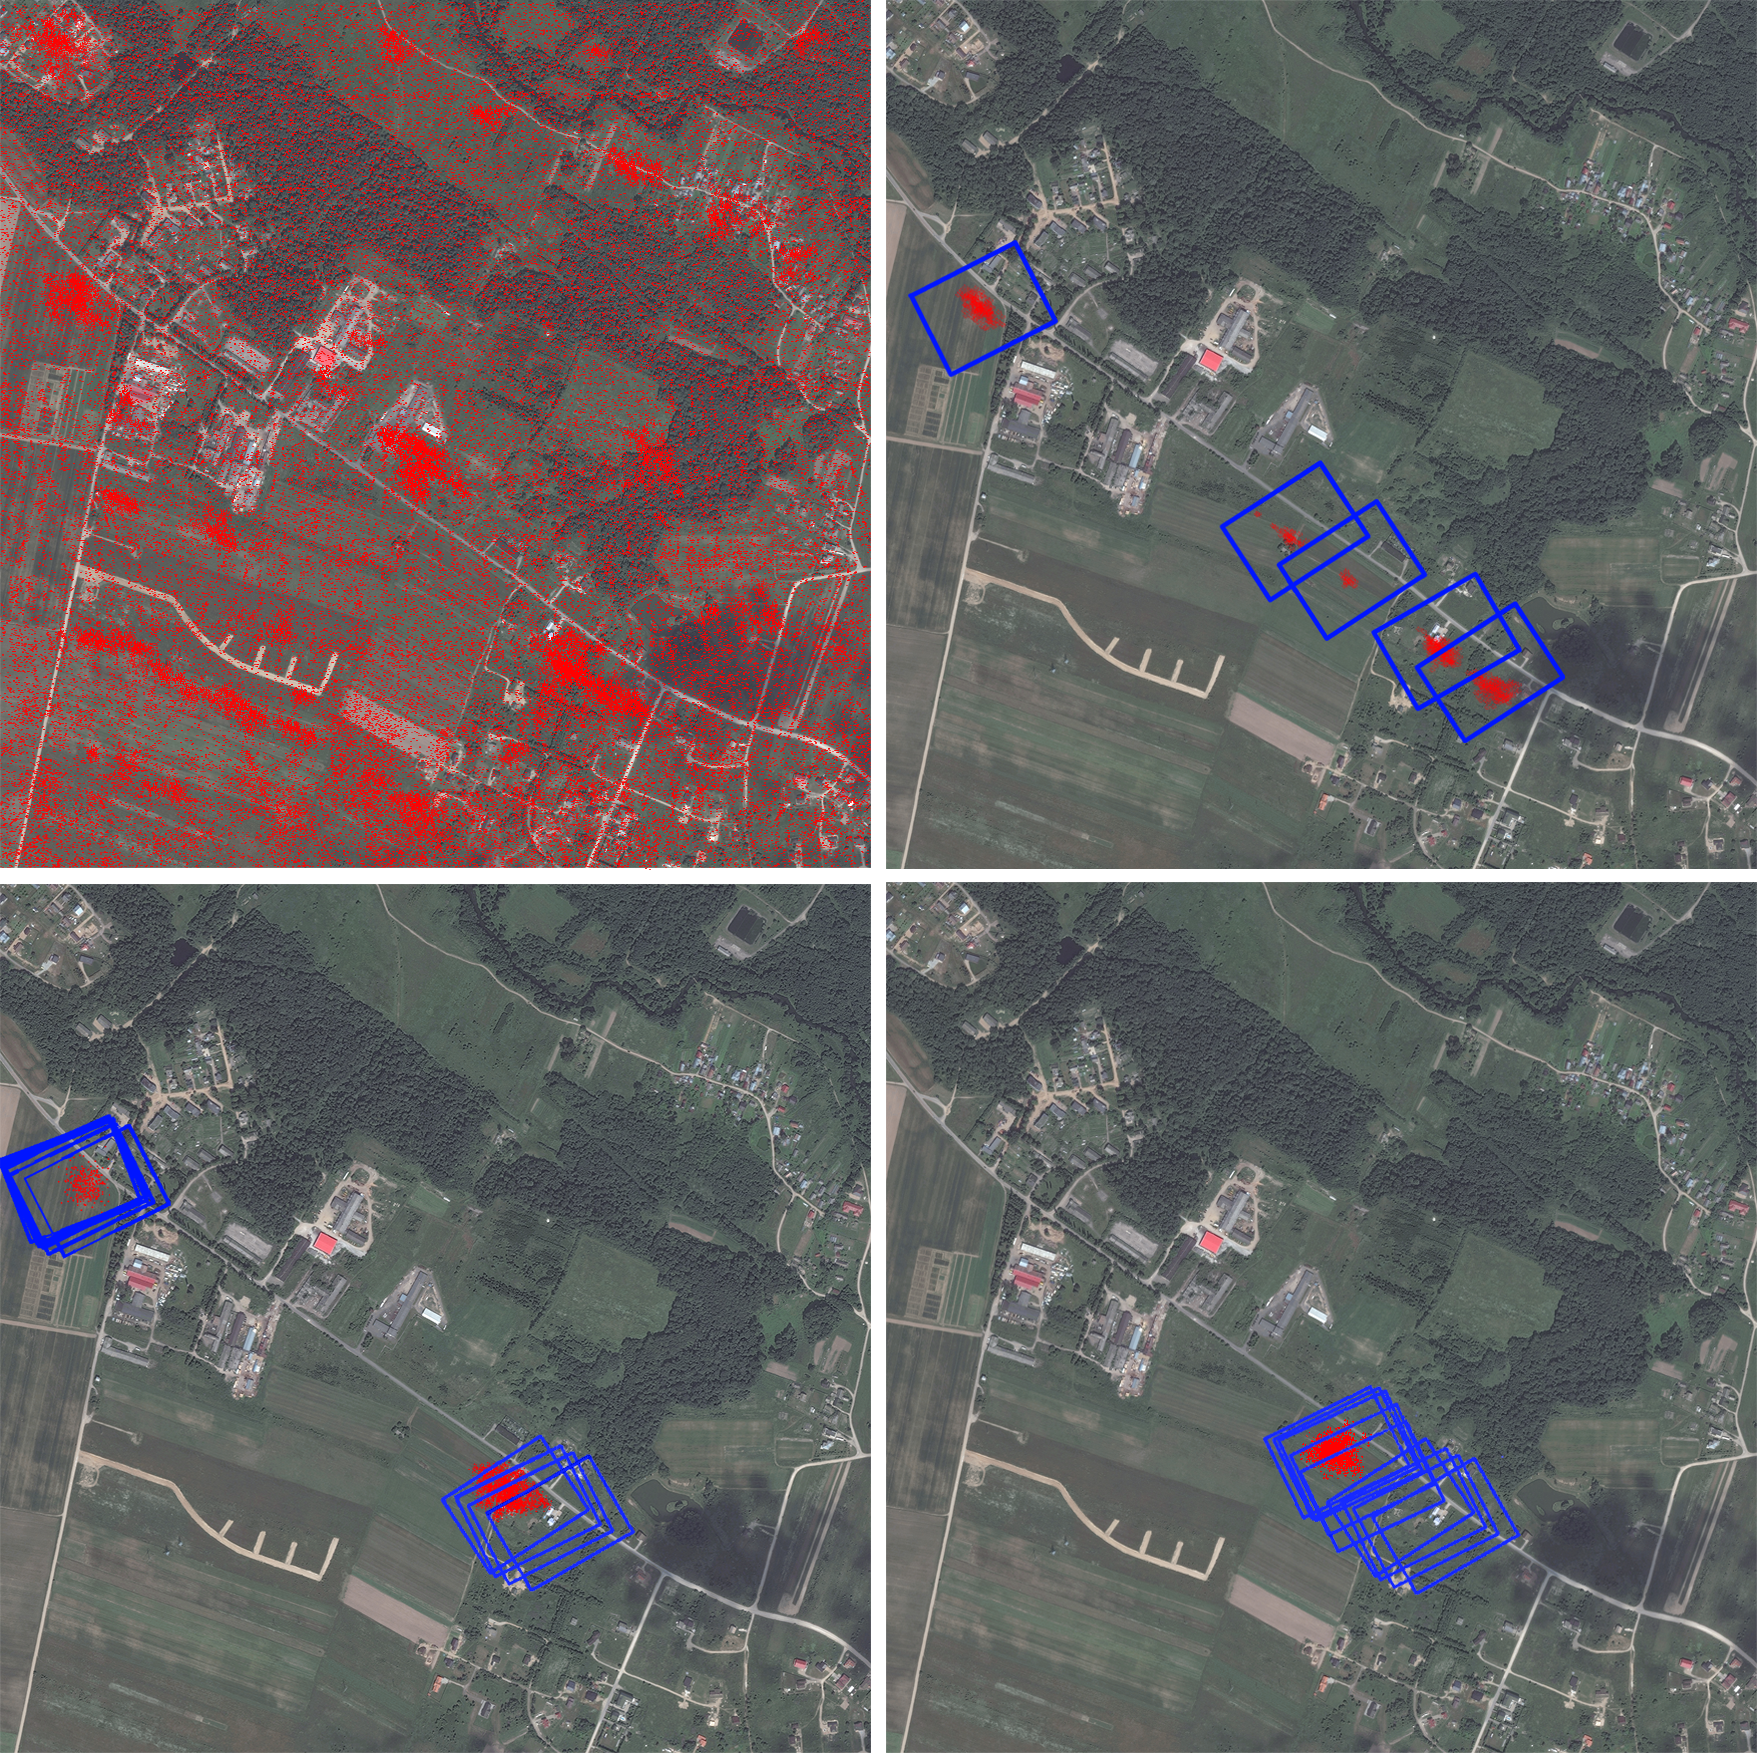
\includegraphics[width=\textwidth]{images/ParticleFilter.png}
				\caption{Dalelių filtro algoritmu yra atliekama lokalizacija žemėlapyje ir iš daugelio įsitikinimų yra išrenkamas vienas. Raudonai yra pažymėtos dalelės, o mėlynais stačiakampiais yra pažymėti suporuoti su žemėlapiu kadrai. Nuo viršaus į dešinę paveikslėliai žymi navigacinės sistemos duomenis: 1) pradinėje stadijoje 2) po 5 kadrų 3) po 50 kadrų 4) po 150 kadrų}
				\label{fig:ParticleFilter}
			\end{figure}
		
		Galiausiai yra apskaičiuojama orlaivio pozicija WGS 84 koordinačių sistemoje. GPS ir vaizdu pagrįstos lokalizacijos rezultatų palyginimas yra pavaizduotas iliustracijoje \ref{fig:localizationsequnce}. Vidutinis skirtumas tarp GPS ir kuriamos navigacinės sistemos duomenų yra 40 metrų. Tačiau galima pastebėti, kad lyginant su GPS visi vaizdu pagrįstos navigacinės sistemos duomenys yra apytiksliai 36 metrais pasislinkę į rytus. Darbo metu šio poslinkio priežastys tiksliai nebuvo nustatytos. 
		
		\begin{figure}[h]
			\centering
			\includegraphics[width=\textwidth]{images/localizationsequnce.png}
			\caption{GPS ir vaizdu pagrįstos navigacinės sistemos rezultatų palyginimas. Mėlynai pažymėtas takas žymi GPS, o raudonai vaizdu pagrįsto navigacinės sistemos duomenis. }
			\label{fig:localizationsequnce}
		\end{figure}
		
	\section{Išvados}
		
			Šio darbo metu buvo sukurta vaizdu paremta vietos nustatymo sistema, kuri dirba kartu su inercine navigacine sistema arba vizualia odometrija. Lokalizacija buvo atlikta tikrų skrydžių simuliacijų metu - t.y. atliekamas skrydis ir vėliau jis yra atkartojama jo simuliacija.		
			Bepilotis orlaivis gali sėkmingai nustatyti savo vietą žemėlapyje, net kai egzistuoja daugiau kaip $9km^2$ neužtikrintumas. Rekursyviai atnaujinant savo poziciją, vaizdu paremta navigacinė sistema geba nustatyti orlaivio koordinates WGS-84 koordinačių sistemoje. Nors vaizdu paremtos navigacinės sistemos duomenys yra nukrypę nuo GPS apskaičiuotų koordinačių vidutiniškai 40 metrų, apytiksliai 36 metrai yra pastovus ir nekintantis nuokrypis, kurį būtų galima pašalinti ateityje.
			Visgi šiai sistemai reikalinga, kur kas didesni skaičiavimo pajėgumai negu remiantis \acrshort{GPS} lokalizacija, taip pat būtina orlaivio atmintyje saugoti geografinius žemėlapius.
			Nepaisant šių trūkumų, vietos nustatymas remiantis vaizdine informacija gali būti viena iš pagrindinių alternatyvų, kaip lokalizuoti bepilotį orlaivį urbanistinėse vietovėse, kur GPS paklaida būna didžiulė ar konfliktinėse zonose.
			
	\subsection{Apribojimai ir galimybės}
	
			Darbo metu naudojamas dalelių filtras yra apibrėžtas 3 dimensijų, kurias sudaro platumos, ilgumos ir posūkio kampai. Esant nedideliam dimensijų skaičiui dalelių filtras rodo puikius rezultatus, tačiau jeigu būtų siekiama išmatuoti orlaivio būsena matuojant daugiau dimensijų, pavyzdžiui, aukštis ar posūkio kampas trijose dimensijos, šis algoritmas reikalautų didelių skaičiavimo pajėgumų.
					
			Daugiausiai skaičiavimo pajėgumų reikalauja paveikslėlių registravimas, tačiau šis algoritmas gali būti skaičiuojamas naudojant vaizdo plokštę.
	\pagebreak
	\section*{Terminai ir trumpiniai}
		\addcontentsline{toc}{section}{Terminai ir trumpiniai}
		\printglossary[title=,toctitle=Terminai ir trumpiniai]
		
		\pagebreak
		\addcontentsline{toc}{section}{Literatūros sąrašas}
		\bibliographystyle{plainlt}
		\bibliography{VisionLocalization}


	\clearpage	  
	\section*{Santrauka}
		\thispagestyle{empty}
		\addcontentsline{toc}{section}{Santrauka}
		
		Globali pozicionavimo sistema (GPS) nėra visada pasiekiama ar saugi naudojimui. Dažniausiai tokia problema iškyla urbanistinėse ar konfliktinėse zonose. 
		Bepiločių orlaivių (BPO) panaudojimo tikslinės sritys dažnai apima vietos nustatymą šiose zonose, todėl šio darbo metu yra apžvelgiamos galimos GPS sistemos alternatyvos, kurios remtųsi vaizdo kamera kaip pagrindiniu jutikliu bei pateikiami pasiūlymai kaip įgyvendinti šią navigacinę sistemą.
		Vaizdo medžiaga iš kameros naudojama susiejant (registruojant) su geografiniu žemėlapiu, taip siekiant nustatyti globalias orlaivio koordinates WGS 84 koordinačių sistemoje. Šios koordinatės yra sujungiamos su inercinės navigacinės sistemos duomenis, taip įgyvendinant pilnavertę navigacinę sistemą.
		Eksperimentiniai  tyrimai, kurių metu buvo simuliacijoje atkuriami tikrų skrydžių duomenys, parodė, kad sistema yra pakankamai tiksli, o paklaida laikui bėgant nesikaupia, todėl ši sistema gali pakeisti GPS ir taip užtikrinti pilną orlaivio autonomiškumą. 
		
	\clearpage
	\section*{Summary}
		\thispagestyle{empty}
		\addcontentsline{toc}{section}{Summary}

		The Global Positioning System (GPS) is not always available and safe to use. Mostly this poblem occurs in urban areas or conflict zones.
		Unmanned aerial vehicles (UAV) taks often includes these areas where UAV possibilities are strongly limited. This work is an overview of possible alternatives to the GPS system, which would use video camera as a primary sensor and proposes how to implement vision-based navigation system.
		Video footage from the camera are registered to the geographical map in order to assess UAV coordinate in WGS-84 coordinate system. These coordinates are combined with data from inertial navigation system. These decisions implements a fully-fledged navigation system.
		Experimental studies, were conducted simulation played real flight data, showed that the system is accurate enough and the error does not accumulate over time, so the system can change the GPS to ensure complete autonomy of the aircraft.

\end{document}